% !TeX spellcheck = it_IT
\section*{Esercizio 1: Simulatore di chiamate a procedura}

	\subsection*{Descrizione ad alto livello}
	
		Iniziamo la descrizione del primo esercizio con la descrizione ad alto livello del codice. La descrizione sarà proposta sia tramite commenti che attraverso dello pseudocodice. All'interno dello pseudocodice verranno definite tutte le procedure definite nel codice assembly, mentre altre funzioni e comandi primitivi, dal significato intuitivo, verranno indicati in blu.
		
		L'idea generale del programma che realizza la soluzione a questo primo esercizio è di analizzare la stringa e, a seconda dell'operazione aritmetica che la caratterizza, invocare l'opportuna procedura. La procedura di ogni operazione si occuperà di estrarre le sotto-stringhe relative ai suoi due operandi e di ricavarne il valore, invocando su di esse, ricorsivamente, la procedura che analizza una stringa. Una volta ricavati i valori degli operandi, ogni procedura potrà combinarli a seconda dell'operazione che implementa e restituire il risultato finale.
		
		Per gestire lo scorrimento della stringa e delle varie sotto-stringhe si è scelto di mantenere due puntatori, uno che punta al primo carattere della stringa in esame ed uno che punta all'ultimo.
		
		Il punto d'entrata del codice è il \pseudo{main()}, descritto qui di seguito:
		
        \begin{center}
           	\begin{lstlisting}[language=pseudo, gobble=14]
                main(){
                    file_descriptor = open("chiamate.txt")
                    buffer_pointer, length = read(file_descriptor)
                    close(file_descriptor)
    	           	
                    start = buffer_pointer + 1
                    end = buffer_pointer + length - 2
                    depth = 0
    	           	
                    analyze(start, end, depth)
    	           	
                    exit
                }
           	\end{lstlisting}
        \end{center}
        
        Come si può intuire, il programma apre il file \bash{chiamate.txt} e ne legge il contenuto. Quindi, calcola i puntatori d'inizio e di fine ed invoca la procedura \pseudo{analyze()} sull'intera stringa. Oltre ai puntatori d'inizio e di fine della stringa, viene mantenuto anche un valore di profondità delle chiamate ricorsive, inizializzato a $0$, utile per stampare i messaggi su consolle con la giusta indentazione.
        
        Di seguito, mostriamo lo pseudocodice della procedura \pseudo{analyze()}:
		
        \begin{center}
           	\begin{lstlisting}[language=pseudo, gobble=14]
                analyze(start, end, depth){
                    char = load_char(start)
    	           	
                    switch(char){
                        case 's':
                            char2 = load_char(start+2)
                            switch(char2):{
                                case 'm':
                                    res = sum(start, end, depth)
                                default:
                                    res = sub(start, end, depth)
                            }
                        case 'p':
                            res = prod(start, end, depth)
                        case 'd':
                            res = div(start, end, depth)
                        default:
                            res = 0
                            while(start < end){
                                digit = load_char(start) - 48
                                res = res + digit
                                res = res * 10
                                start = start + 1
                            }
                            digit = load_char(start) - 48
                            res = res + digit
                    }
                    
                    return res
                }
           	\end{lstlisting}
        \end{center}
        
        Il compito della funzione \pseudo{analyze()} è quello di determinare quale operazione aritmetica caratterizza la stringa passata in input (ovvero la stringa delimitata dai puntatori \pseudo{start} ed \pseudo{end} passati come parametri). Dal momento che si assume che la stringa descritta in \bash{chiamate.txt} sia sempre sintatticamente corretta, per determinare l'operazione principale della stringa basterà analizzare il primo carattere: se è $s$ allora è o una somma o una sottrazione (in questo caso esamina il terzo carattere), se è $p$ allora è un prodotto, se è $d$ allora è una divisione, altrimenti è un valore già ridotto a intero.
        
        Una volta individuata l'operazione, si passano gli stessi parametri passati ad \pseudo{analyze()} alla funzione corrispondente all'operazione. Il risultato di questa chiamata a funzione sarà poi restituito a sua volta da \pseudo{analyze()}.
        
        Nel caso di un valore intero, per poter calcolare il valore di ritorno è necessario effettuare un'operazione di parsing da una serie di caratteri (le cifre che compongono il numero nella stringa) ad un intero. Per fare questo viene innanzitutto caricato ogni carattere, corrispondente ad una cifra, e viene convertito in intero sottraendovi $48$ al suo valore numerico: questo viene fatto in quanto, all'interno della codifica ASCII, le cifre vengono codificate a partire dal valore decimale $48$ (corrispondente allo $0$) fino a $57$ (corrispondente al carattere $9$)\footnote{Si veda la discussione all'indirizzo \url{http://www.dreamincode.net/forums/topic/284141-how-to-convert-a-char-into-int/}.}. A questo punto, se ancora non si è raggiunto l'ultimo carattere, si somma tale valore al numero fin'ora calcolato (inizializzato a $0$) e si moltiplica il tutto per $10$ (ovvero shiftando, di fatto, di una posizione verso sinistra il valore decimale del numero). Infine, una volta trovata l'ultima cifra, si somma al numero calcolato (senza moltiplicare per $10$, essendo le unità) ottenendo il valore finale rappresentato come intero.
        
        Vediamo adesso, di seguito, lo pseudocodice corrispondente alle quattro operazioni aritmetiche:
        
        \begin{center}
           	\begin{lstlisting}[language=pseudo, gobble=14]
                sum(start, end, depth){
                   	print_call(start, end, depth)
                   	
                   	start = start + 6
                   	end = end - 1
                   	
                   	op1, op2 = get_operands(start, end, depth)
                   	res = op1 + op2
                   	
                   	print_return("somma-return", res, depth)
                   	
                   	return res
                }
                
                sub(start, end, depth){
                   	print_call(start, end, depth)
                   	
                   	start = start + 12
                   	end = end - 1
                   	
                   	op1, op2 = get_operands(start, end, depth)
                   	res = op1 - op2
                   	
                   	print_return("sottrazione-return", res, depth)
                   	
                   	return res
                }
                
                prod(start, end, depth){
                   	print_call(start, end, depth)
                   	
                   	start = start + 9
                   	end = end - 1
                   	
                   	op1, op2 = get_operands(start, end, depth)
                   	res = op1 * op2
                   	
                   	print_return("prodotto-return", res, depth)
                   	
                   	return res
                }
                
                div(start, end, depth){
                   	print_call(start, end, depth)
                   	
                   	start = start + 10
                   	end = end - 1
                   	
                   	op1, op2 = get_operands(start, end, depth)
                   	res = op1 / op2
                   	
                   	print_return("divisione-return", res, depth)
                   	
                   	return res
                }
           	\end{lstlisting}
        \end{center}
        
        Le implementazioni delle quattro operazioni sono molto simili e si distinguono soltanto per alcuni dettagli. Innanzitutto viene invocata la procedura \pseudo{print_call()} sugli stessi parametri di input: questa funzione permette di stampare su console la riga corrispondente alla chiamata a procedura. Dopodiché vengono aggiornati i puntatori d'inizio e di fine della stringa saltando il nome dell'operazione in testa e l'apertura e chiusura delle parentesi: il puntatore finale viene sempre decrementato di $1$ (per saltare la chiusura di parentesi finale) mentre i caratteri da saltare all'inizio variano a seconda dell'operazione (ad esempio per la somma si deve saltare $somma($, ovvero $6$ caratteri, come vediamo in riga 4 del codice, mentre per la sottrazione si salta $sottrazione($, ovvero $12$ caratteri totali, come si vede in riga 18). A questo punto si invoca la funzione \pseudo{get_operands()}, sui nuovi puntatori aggiornati e sulla stessa profondità, che si occupa di calcolare il valore intero dei due operandi coinvolti nell'operazione e restituirli. Una volta ottenuti gli operandi, si può effettuare l'operazione richiesta (somma, sottrazione, ecc\dots). Quindi verrà invocata la procedura \pseudo{print_return()} la quale, data una stringa caratterizzante l'operazione, il risultato calcolato e la profondità, stampa il messaggio su console relativo al ritorno della procedura. Infine la funzione restituisce il valore calcolato.
        
        Vediamo di seguito l'implementazione in pseudocodice della funzione \pseudo{get_operands()}:
        
        \begin{center}
           	\begin{lstlisting}[language=pseudo, gobble=14]
                get_operands(start, end, depth){
                    depth = depth + 1
                    i = start
                    pars = 0
                    while(true){
                        char = load_char(i)
                        switch(char){
                            case '(':
                                pars = pars + 1
                            case ')':
                                pars = pars - 1
                            case ',':
                                if(pars == 0){
                                    break
                                }
                        }
                        i = i + 1
                    }
                    res1 = analyze(start, i-1, depth)
                    res2 = analyze(i+1, end, depth)
                    return res1, res2
                }
           	\end{lstlisting}
        \end{center}
        
        La funzione che estrae il valore degli operandi incrementa, innanzitutto, la profondità di chiamata di $1$: infatti, quando si effettueranno le chiamate ricorsive sui due operandi, queste avranno una profondità maggiore rispetto alla chiamata ``padre''. Quindi, viene creato un puntatore \pseudo{i}, inizializzato col puntatore d'inizio, ed un contatore \pseudo{pars}, inizializzato a $0$, che conta il numero di parentesi aperte ma non chiuse.
        
        Dopodiché si inizia un ciclo. Il ciclo consiste nel caricare il carattere attualmente puntato dal puntatore \pseudo{i} e controllare, innanzitutto, che non sia una parentesi, nel qual caso incrementa o decrementa \pseudo{pars} di conseguenza e incrementa \pseudo{i}. Se il carattere è invece una virgola, controlla allora se \pseudo{pars} è $0$: in questo caso si è trovata la posizione della virgola che separa i due operandi dell'operazione più esterna, in caso contrario, invece, è la virgola di un'operazione più interna, che non ci interessa al momento.
        
        Una volta trovata al virgola che divide gli operandi dell'operazione in esame si esce dal ciclo e si possono invocare le chiamate ricorsive sui due operandi per ottenerne i valori: il primo è delimitato dal puntatore d'inizio e dal puntatore precedente a quello della virgola, mentre il secondo è delimitato dal puntatore successivo alla virgola e dal puntatore di fine. I due valori verranno quindi restituiti, in modo da poter essere combinati opportunamente dalla funzione dell'operazione aritmetica, come visto prima.
        
        Infine, vediamo l'implementazione delle due funzioni ausiliarie \pseudo{print_call()} e \pseudo{print_return()}:
		
        \begin{center}
           	\begin{lstlisting}[language=pseudo, gobble=14]
                print_call(start, end, depth){
                    while(depth > 0){
                        print_tab()
                        depth = depth - 1
                    }
                    print("-->")
                    while(start <= end){
                        char = load_char(start)
                        print(char)
                        start = start + 1
                    }
                    print_newline()
                }
                
                print_return(return_string, res, depth){
                    while(depth > 0){
                        print_tab()
                        depth = depth - 1
                    }
                    print("<--" + return_string + "(" + res + ")")
                    print_newline()
                }
           	\end{lstlisting}
        \end{center}
		
		Entrambe le procedure iniziano stampando un numero di tabulazioni pari alla profondità di chiamata. Dopodiché viene stampata la freccia, verso destra o verso sinistra, a seconda che sia l'invocazione o la terminazione di una chiamata, rispettivamente. Infine, per l'invocazione di chiamata, viene effettuato un ciclo per stampare l'intera stringa attuale, mentre per la terminazione di chiamata viene stampata la stringa caratteristica dell'operazione (ad esempio \pseudo{"somma-return"} per la somma) e quindi il valore del risultato tra parentesi.
		
	\subsection*{Motivazione delle scelte implementative}
		La principale scelta implementativa, ovvero mantenere di volta in volta i puntatori d'inizio e di fine, è stata una scelta dettata dalla semplicità e dalla facilità d'implementazione, nonché da motivazioni legate alla performance del codice. Una possibile alternativa sarebbe infatti potuta essere quella di andare effettivamente di volta in volta a modificare la stringa, shiftandola verso sinistra per eliminare i caratteri in testa e shiftando a sinistra il carattere di terminazione della stringa per eliminare i caratteri in coda. Questa soluzione alternativa sarebbe risultata chiaramente più macchinosa e difficile da implementare, nonché più pesante a livello di esecuzione, dovendo ogni volta, anche per eliminare un solo carattere, shiftare l'intera stringa, rendendo ogni operazione sulla stringa un'operazione di complessità $\mathcal{O}(n)$, con $n$ lunghezza della stringa. Lavorando sui puntatori, invece, ogni operazione sulla stringa ha costo lineare $\mathcal{O}(1)$ e l'implementazione di questa strategia è sicuramente più semplice e leggibile, in quanto uno shift della stringa di qualsiasi tipo corrisponde al semplice incremento/decremento del puntatore corrispondente. La stringa viene allocata, per comodità, nella sezione della memoria statica, assumendo un massimo di $1024$ byte, ovvero $1024$ caratteri.
		
		Prima di ogni chiamata a procedura, come da convenzione, viene allocato spazio sufficiente nello stack frame, in modo da poter memorizzare e ``mettere al sicuro'' i valori che si intende recuperare dopo la terminazione della procedura invocata.
		
		Infine, in alcuni punti, come ad esempio all'inizio di una procedura, vengono fatte delle copie, da un registro ad un altro, che in alcuni casi possono sembrare anche troppo ridondanti o inutili. Questa scelta è stata fatta in modo da rendere il codice più leggibile ma soprattutto per seguire nel modo più rigoroso possibile le convenzioni sull'uso dei registri: in alcuni casi, ad esempio, si potrebbe lavorare direttamente su registri come \mips{\$a0}, \mips{\$a1} o \mips{\$v0}, ma le convenzioni impongono che tali registri sono riservati agli input e agli output, ed è quindi necessario, nel caso si volesse lavorare con valori contenuti in essi, copiarne preventivamente il contenuto su registri temporanei, come \mips{\$t0} e quindi effettuare le operazioni necessarie.
		
	\subsection*{Simulazioni}
		Mostriamo adesso un paio di esecuzioni tipo del programma. Dal momento che si assume che le stringhe di input siano sempre sintatticamente corrette, non verranno presi in esame situazioni di errore in cui le stringhe inserite hanno sintassi scorrette. Verranno invece mostrati gli output per le tre stringhe proposte nel testo dell'esercizio.
		
       	\begin{figure}[h!]
       		\begin{center}
       			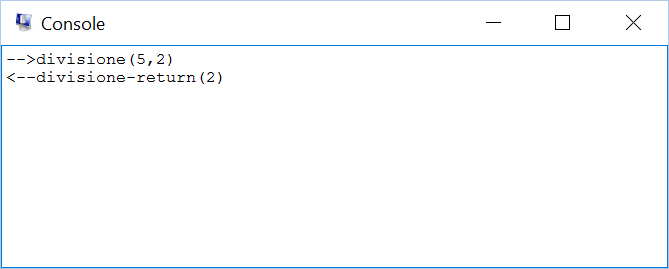
\includegraphics[scale=1]{es1_small.png}
       		\end{center}
       		\caption{Output con la stringa \textit{"divisione(5,2)"}.}
       		\label{fig:es1_small}
       	\end{figure}
       	
       	\begin{figure}[h!]
       		\begin{center}
       			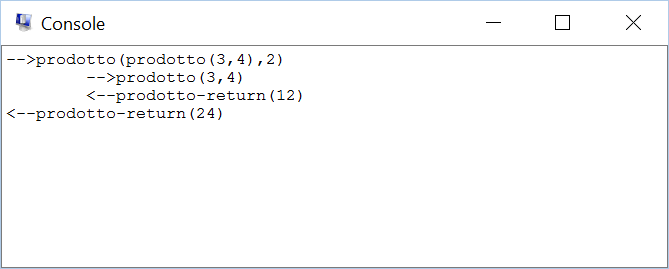
\includegraphics[scale=1]{es1_medium.png}
       		\end{center}
       		\caption{Output con la stringa \textit{"prodotto(prodotto(3,4),2)"}.}
       		\label{fig:es1_medium}
       	\end{figure}
       	
       	\begin{figure}[h!]
       		\begin{center}
       			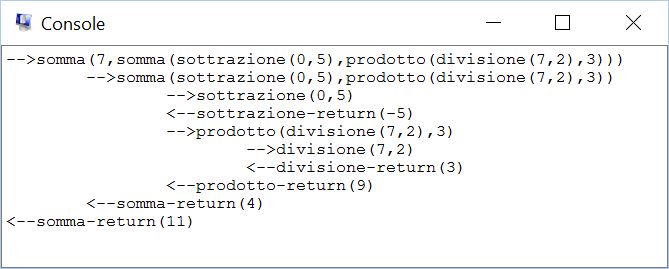
\includegraphics[scale=1]{es1_big.png}
       		\end{center}
       		\caption{Output con la stringa \textit{"somma(7,somma(sottrazione(0,5),prodotto(divisione(7,2),3)))"}.}
       		\label{fig:es1_big}
       	\end{figure}
       	
       	Come possiamo notare dalle Figure dalla \ref{fig:es1_small} alla \ref{fig:es1_big}, i risultati stampati su consolle sono esattamente quelli attesi, indice che il programma funziona correttamente per input dalle dimensioni più svariate. Inoltre si può notare come l'indentazione delle varie chiamate sia stata implementata con successo, rendendo l'output più chiaro ed intuitivo.
       	
       	\FloatBarrier
       	
    \subsection*{Codice MIPS}
		
		Di seguito, il codice MIPS completo che implementa il programma descritto dall'esercizio 1, opportunamente commentato.
		
        \begin{center}
           	\begin{lstlisting}[language=mips, gobble=14, stepnumber=1]
                # Title: Simulatore di chiamate a procedura     Filename: es1.s
                # Author1: ??? ?????    ???????     ???.?????@stud.unifi.it
                # Author2: ??? ?????    ???????     ???.?????@stud.unifi.it
                # Author3: ??? ?????    ???????     ???.?????@stud.unifi.it
                # Date: ??/??/????
                # Description:  Chiamate a procedura per l'esecuzione di operazioni aritmetiche
                # Input: chiamate.txt
                # Output: Traccia delle chiamate su console
                
                ################# Data segment #####################
                .data
                file:           .asciiz "chiamate.txt"
                tab:            .asciiz "\t"
                newline:        .asciiz "\n"
                arrow_r:        .asciiz "-->"
                arrow_l:        .asciiz "<--"
                buffer:         .space  1024
                sum_return:     .asciiz "somma-return"
                sub_return:     .asciiz "sottrazione-return"
                prod_return:    .asciiz "prodotto-return"
                div_return:     .asciiz "divisione-return"
                
                ################# Code segment #####################
                .text
                .globl main
                
                ### Print call ###
                print_call:
                    move $t0, $a0   # copia i tre parametri in registri temporanei
                    move $t1, $a1
                    move $t2, $a2
                    
                print_call_tabs:
                    beq $t2, $zero, print_call_arrow    # se la profondità è 0, allora procede a stampare la stringa
                                                        # altrimenti
                    li $v0, 4   # stampa una tabulazione
                    la $a0, tab
                    syscall
                    
                    addi $t2, $t2, -1   # decrementa la profondità
                    
                    j print_call_tabs   # ed esegue un altro ciclo
                    
                print_call_arrow:
                    li $v0, 4       # stampa la freccia verso destra
                    la $a0, arrow_r
                    syscall
                    
                print_call_string:
                    li $v0, 11      # stampa il carattere puntato da $a0
                    lb $a0, 0($t0)
                    syscall
                    
                    beq $t0, $t1, print_call_done   # se i puntatori d'inizio e di fine coincidono allora la stringa è finita
                    
                    addi $t0, $t0, 1    # altrimenti incrementa il puntatore d'inizio (scorre al prossimo carattere)
                    
                    j print_call_string # ed esegue un altro ciclo
                    
                print_call_done:
                    li $v0, 4       # alla fine stampa una newline (a capo)
                    la $a0, newline
                    syscall
                    
                    jr $ra  # e torna al chiamante
                ### Print call end ###
                
                ### Print return ###
                print_return:
                    move $t0, $a0   # copia i tre parametri in registri temporanei
                    move $t1, $a1
                    move $t2, $a2
                    
                print_return_tabs:  # analogo a print_call_tabs
                    beq $t2, $zero, print_return_string
                    
                    li $v0, 4
                    la $a0, tab
                    syscall
                    
                    addi $t2, $t2, -1
                    
                    j print_return_tabs
                    
                print_return_string:
                    li $v0, 4       # stampa la freccia verso sinistra
                    la $a0, arrow_l
                    syscall
                    move $a0, $t0   # stampa la stringa di ritorno relativa all'operazione
                    syscall
                    li $v0, 11      # stampa il simbolo di aperta parentesi
                    li $a0, '('
                    syscall
                    li $v0, 1       # stampa il risultato dell'operazione
                    move $a0, $t1
                    syscall
                    li $v0, 11      # stampa il simbolo di chiusa parentesi
                    li $a0, ')'
                    syscall
                    li $v0, 4       # stampa una newline (a capo)
                    la $a0, newline
                    syscall
                    
                    jr $ra  # infine torna al chiamante
                ### Print return end ###
                
                ### Get operands ###
                get_operands:
                    addi $sp, $sp, -20  # alloca spazio per 5 words nello stack frame
                    sw $ra, 16($sp)     # salva l'indirizzo di ritorno
                    sw $a1, 12($sp)     # il puntatore di fine
                    addi $a2, $a2, 1    # e la profondità della chiamata incrementata di 1
                    sw $a2, 8($sp)
                    
                    move $t0, $a0   # inizializza $t0 con il puntatore d'inizio
                    move $t1, $zero # e $t1 con 0 ($t1 indica il numero di parentesi aperte ma non ancora chiuse)
                    
                get_operands_search:
                    lb $t3, 0($t0)                      # carica il carattere puntato da $t0
                    li $t4, '('
                    beq $t3, $t4, get_operands_open     # controlla se è una parentesi aperta
                    li $t4, ')'
                    beq $t3, $t4, get_operands_close    # una parentesi chiusa
                    li $t4, ','
                    beq $t3, $t4, get_operands_comma    # oppure una virgola
                    j get_operands_advance              # altrimenti va avanti senza fare niente
                    
                get_operands_open:
                    addi $t1, $t1, 1        # se si trova una parentesi aperta si incremente $t1
                    j get_operands_advance  # e si passa al prossimo carattere
                    
                get_operands_close:
                    addi $t1, $t1, -1       # se si trova una parentesi chiusa si decremente $t1
                    j get_operands_advance  # e si passa al prossimo carattere
                    
                get_operands_comma:
                    beq $t1, $zero, get_operands_found  # se si trova una virgola e le parentesi sono bilanciate, allora si è trovato il punto di divisione
                    j get_operands_advance              # altrimenti si passa al prossimo carattere
                    
                get_operands_advance:
                    addi $t0, $t0, 1        # incrementa di 1 il puntatore $t0
                    j get_operands_search   # e continua la ricerca
                    
                get_operands_found:
                    sw $t0, 4($sp)  # salva il puntatore alla virgola nello stack
                    
                    addi $t0, $t0, -1   # decrementa il puntatore $t0 (carattere subito prima della virgola)
                    move $a1, $t0       # e lo imposta come secondo parametro per analyze
                    
                    jal analyze # invoca analyze sul primo operando con profondità incrementata di 1
                    
                    sw $v0, 0($sp)  # salva il valore del primo operando nello stack
                    
                    lw $a0, 4($sp)      # recupera il puntatore alla virgola
                    addi $a0, $a0, 1    # e lo imposta come primo parametro (puntatore d'inizio) incrementandolo di 1 (primo carattere dopo la virgola)
                    lw $a1, 12($sp)     # recupera il puntatore di fine
                    lw $a2, 8($sp)      # recupera la profondità incrementata di 1
                    
                    jal analyze # invoca analyze sul primo operando con profondità incrementata di 1
                    
                    move $v1, $v0   # salva il valore del secondo operando come secondo risultato
                    lw $v0, 0($sp)  # recupera il valore del primo operando e lo imposta come primo risultato
                    
                    lw $ra, 16($sp)     # recupera l'indirizzo di ritorno
                    addi $sp, $sp, 20   # dealloca lo stack frame
                    jr $ra              # ritorna al chiamante
                ### Get operands end ###
                
                ### Call sum ###
                call_sum:
                    addi $sp, $sp, -20  # alloca spazio per cinque words nello stack frame
                    sw $ra, 16($sp)     # salva l'indirizzo di ritorno nello stack
                    
                    move $t0, $a0   # primo parametro: puntatore d'inizio
                    move $t1, $a1   # secondo: puntatore di fine
                    move $t2, $a2   # terzo: profondità della chiamata
                    
                    sw $t0, 12($sp)     # il puntatore d'inizio
                    sw $t1, 8($sp)      # il puntatore di fine
                    sw $t2, 4($sp)      # e la profondità della chiamata
                    
                    move $a0, $t0   # primo parametro: puntatore d'inizio
                    move $a1, $t1   # secondo: puntatore di fine
                    move $a2, $t2   # terzo: profondità della chiamata
                    
                    jal print_call      # invoca la procedura per la stampa dell'invocazione (con gli stessi parametri)
                    
                    lw $t0, 12($sp)     # recupera il puntatore d'inizio dallo stack
                    addi $t0, $t0, 6    # salta la stringa "somma(" (6 caratteri)
                    lw $t1, 8($sp)      # recupera il puntatore di fine
                    addi $t1, $t1, -1   # scarta l'ultima parentesi chiusa
                    lw $t2, 4($sp)      # recupera la profondità della chiamata
                    
                    move $a0, $t0   # primo parametro: puntatore d'inizio
                    move $a1, $t1   # secondo: puntatore di fine
                    move $a2, $t2   # terzo: profondità della chiamata
                    
                    jal get_operands    # invoca la procedura per ottenere gli operandi
                    
                    move $t0, $v0   # primo valore di ritorno: valore del primo operando
                    move $t1, $v1   # secondo: valore del secondo operando
                    
                    add $t2, $t0, $t1   # somma i due operandi ottenuti
                    sw $t2, 0($sp)      # salva il risultato nello stack
                    
                    la $a0, sum_return  # carica l'indirizzo della stringa sum_return (primo parametro)
                    move $a1, $t2       # imposta il risultato dell'operazione come secondo parametro
                    lw $a2, 4($sp)      # recupera la profondità della chiamata (terzo parametro)
                    
                    jal print_return    # invoca la stampa del risultato con questi tre parametri
                    
                    lw $v0, 0($sp)      # recupera il risultato dell'operazione
                    lw $ra, 16($sp)     # recupera l'indirizzo di ritorno
                    addi $sp, $sp, 20   # dealloca lo stack frame
                    jr $ra              # torna al chiamante
                ### Call sum end ###
                
                ### Call subtraction ###
                call_sub:
                    addi $sp, $sp, -20  # alloca spazio per cinque words nello stack frame
                    sw $ra, 16($sp)     # salva l'indirizzo di ritorno nello stack
                    
                    move $t0, $a0   # primo parametro: puntatore d'inizio
                    move $t1, $a1   # secondo: puntatore di fine
                    move $t2, $a2   # terzo: profondità della chiamata
                    
                    sw $t0, 12($sp)     # il puntatore d'inizio
                    sw $t1, 8($sp)      # il puntatore di fine
                    sw $t2, 4($sp)      # e la profondità della chiamata
                    
                    move $a0, $t0   # primo parametro: puntatore d'inizio
                    move $a1, $t1   # secondo: puntatore di fine
                    move $a2, $t2   # terzo: profondità della chiamata
                    
                    jal print_call      # invoca la procedura per la stampa dell'invocazione (con gli stessi parametri)
                    
                    lw $t0, 12($sp)     # recupera il puntatore d'inizio dallo stack
                    addi $t0, $t0, 12   # salta la stringa "sottrazione(" (12 caratteri)
                    lw $t1, 8($sp)      # recupera il puntatore di fine
                    addi $t1, $t1, -1   # scarta l'ultima parentesi chiusa
                    lw $t2, 4($sp)      # recupera la profondità della chiamata
                    
                    move $a0, $t0   # primo parametro: puntatore d'inizio
                    move $a1, $t1   # secondo: puntatore di fine
                    move $a2, $t2   # terzo: profondità della chiamata
                    
                    jal get_operands    # invoca la procedura per ottenere gli operandi
                    
                    move $t0, $v0   # primo valore di ritorno: valore del primo operando
                    move $t1, $v1   # secondo: valore del secondo operando
                    
                    sub $t2, $t0, $t1   # sottrae il secondo operando al primo
                    sw $t2, 0($sp)      # salva il risultato nello stack
                    
                    la $a0, sub_return  # carica l'indirizzo della stringa sub_return (primo parametro)
                    move $a1, $t2       # imposta il risultato dell'operazione come secondo parametro
                    lw $a2, 4($sp)      # recupera la profondità della chiamata (terzo parametro)
                    
                    jal print_return    # invoca la stampa del risultato con questi tre parametri
                    
                    lw $v0, 0($sp)      # recupera il risultato dell'operazione
                    lw $ra, 16($sp)     # recupera l'indirizzo di ritorno
                    addi $sp, $sp, 20   # dealloca lo stack frame
                    jr $ra              # torna al chiamante
                ### Call subtraction end ###
                
                ### Call product ###
                call_prod:
                    addi $sp, $sp, -20  # alloca spazio per cinque words nello stack frame
                    sw $ra, 16($sp)     # salva l'indirizzo di ritorno nello stack
                    
                    move $t0, $a0   # primo parametro: puntatore d'inizio
                    move $t1, $a1   # secondo: puntatore di fine
                    move $t2, $a2   # terzo: profondità della chiamata
                    
                    sw $t0, 12($sp)     # il puntatore d'inizio
                    sw $t1, 8($sp)      # il puntatore di fine
                    sw $t2, 4($sp)      # e la profondità della chiamata
                    
                    move $a0, $t0   # primo parametro: puntatore d'inizio
                    move $a1, $t1   # secondo: puntatore di fine
                    move $a2, $t2   # terzo: profondità della chiamata
                    
                    jal print_call      # invoca la procedura per la stampa dell'invocazione (con gli stessi parametri)
                    
                    lw $t0, 12($sp)     # recupera il puntatore d'inizio dallo stack
                    addi $t0, $t0, 9    # salta la stringa "prodotto(" (9 caratteri)
                    lw $t1, 8($sp)      # recupera il puntatore di fine
                    addi $t1, $t1, -1   # scarta l'ultima parentesi chiusa
                    lw $t2, 4($sp)      # recupera la profondità della chiamata
                    
                    move $a0, $t0   # primo parametro: puntatore d'inizio
                    move $a1, $t1   # secondo: puntatore di fine
                    move $a2, $t2   # terzo: profondità della chiamata
                    
                    jal get_operands    # invoca la procedura per ottenere gli operandi
                    
                    move $t0, $v0   # primo valore di ritorno: valore del primo operando
                    move $t1, $v1   # secondo: valore del secondo operando
                    
                    mul $t2, $t0, $t1   # moltiplica i due operandi ottenuti
                    sw $t2, 0($sp)      # salva il risultato nello stack
                    
                    la $a0, prod_return # carica l'indirizzo della stringa prod_return (primo parametro)
                    move $a1, $t2       # imposta il risultato dell'operazione come secondo parametro
                    lw $a2, 4($sp)      # recupera la profondità della chiamata (terzo parametro)
                    
                    jal print_return    # invoca la stampa del risultato con questi tre parametri
                    
                    lw $v0, 0($sp)      # recupera il risultato dell'operazione
                    lw $ra, 16($sp)     # recupera l'indirizzo di ritorno
                    addi $sp, $sp, 20   # dealloca lo stack frame
                    jr $ra              # torna al chiamante
                ### Call product end ###
                
                ### Call division ###
                call_div:
                    addi $sp, $sp, -20  # alloca spazio per cinque words nello stack frame
                    sw $ra, 16($sp)     # salva l'indirizzo di ritorno nello stack
                    
                    move $t0, $a0   # primo parametro: puntatore d'inizio
                    move $t1, $a1   # secondo: puntatore di fine
                    move $t2, $a2   # terzo: profondità della chiamata
                    
                    sw $t0, 12($sp)     # il puntatore d'inizio
                    sw $t1, 8($sp)      # il puntatore di fine
                    sw $t2, 4($sp)      # e la profondità della chiamata
                    
                    move $a0, $t0   # primo parametro: puntatore d'inizio
                    move $a1, $t1   # secondo: puntatore di fine
                    move $a2, $t2   # terzo: profondità della chiamata
                    
                    jal print_call      # invoca la procedura per la stampa dell'invocazione (con gli stessi parametri)
                    
                    lw $t0, 12($sp)     # recupera il puntatore d'inizio dallo stack
                    addi $t0, $t0, 10   # salta la stringa "divisione(" (10 caratteri)
                    lw $t1, 8($sp)      # recupera il puntatore di fine
                    addi $t1, $t1, -1   # scarta l'ultima parentesi chiusa
                    lw $t2, 4($sp)      # recupera la profondità della chiamata
                    
                    move $a0, $t0   # primo parametro: puntatore d'inizio
                    move $a1, $t1   # secondo: puntatore di fine
                    move $a2, $t2   # terzo: profondità della chiamata
                    
                    jal get_operands    # invoca la procedura per ottenere gli operandi
                    
                    move $t0, $v0   # primo valore di ritorno: valore del primo operando
                    move $t1, $v1   # secondo: valore del secondo operando
                    
                    div $t2, $t0, $t1   # divide (operazione quoziente) il primo operando per il secondo
                    sw $t2, 0($sp)      # salva il risultato nello stack
                    
                    la $a0, div_return  # carica l'indirizzo della stringa div_return (primo parametro)
                    move $a1, $t2       # imposta il risultato dell'operazione come secondo parametro
                    lw $a2, 4($sp)      # recupera la profondità della chiamata (terzo parametro)
                    
                    jal print_return    # invoca la stampa del risultato con questi tre parametri
                    
                    lw $v0, 0($sp)      # recupera il risultato dell'operazione
                    lw $ra, 16($sp)     # recupera l'indirizzo di ritorno
                    addi $sp, $sp, 20   # dealloca lo stack frame
                    jr $ra              # torna al chiamante
                ### Call division end ###
                    
                ### Analyze ###
                analyze:
                    addi $sp, $sp, -4  # alloca spazio per una word nello stack frame
                    sw $ra, 0($sp)     # salva l'indirizzo di ritorno del chiamante
                
                    # i parametri di input delle chiamate sono gli stessi di analyze, ovvero:
                    # primo: puntatore d'inizio
                    # secondo: puntatore di fine
                    # terzo: profondità della chiamata
                    
                    lb $t0, 0($a0)                  # carica il primo carattere della stringa
                    li $t1, 's'                     # se è 's'
                    beq $t0, $t1, analyze_sum_sub   # allora è una somma o una sottrazione
                    li $t1, 'p'                     # se è 'p'
                    beq $t0, $t1, jump_prod         # allora è un prodotto
                    li $t1, 'd'                     # se è 'd'
                    beq $t0, $t1, jump_div          # allora è una divisione
                    j analyze_int                   # altrimenti è già un intero
                    
                analyze_sum_sub:
                    lb $t0, 2($a0)           # carica il terzo carattere della stringa
                    li $t1, 'm'              # se è 'm'
                    beq $t0, $t1, jump_sum   # allora è una somma
                    j jump_sub               # altrimenti è una sottrazione
                    
                jump_sum:
                    jal call_sum    # invoca la procedura relativa alla somma
                    j analyze_end   # quando ritorna invoca la fine dell'analisi (comune a tutte le operazioni)
                    
                jump_sub:           # sub, prod e div analoghe a sum
                    jal call_sub
                    j analyze_end
                    
                jump_prod:
                    jal call_prod
                    j analyze_end
                    
                jump_div:
                    jal call_div
                    j analyze_end
                    
                analyze_int:
                    move $v0, $zero #inizializza il valore dell'intero a 0
                    
                analyze_int_loop:
                    lb $t1, 0($a0)      # carica il carattere puntato da $a0
                    addi $t1, $t1, -48  # sottrae 48 (parsing da codifica ASCII a intero)
                    add $v0, $v0, $t1   # somma la cifra ottenuta ($t1) col valore fin'ora calcolato ($v0)
                    
                    beq $a0, $a1, analyze_end   # se i puntatori d'inizio e fine coincidono allora era l'ultimo carattere
                                                # altrimenti
                    li $t2, 10
                    mul $v0, $v0, $t2   # moltiplica il valore fin'ora calcolato per 10
                    addi $a0, $a0, 1    # incrementa il puntatore di 1 (prossimo carattere)
                    
                    j analyze_int_loop  # ed esegue un altro ciclo
                    
                analyze_end:
                    # nel caso delle chiamate a procedura, il valore di ritorno è lo stesso (valutazione dell'espressione)
                    lw $ra, 0($sp)      # recupera l'indirizzo di ritorno
                    addi $sp, $sp, 4    # dealloca lo stack
                    jr $ra              # torna al chiamante
                ### Analyze end ###
                
                ### Main ###
                main:
                    li $v0, 13      # apre il file (syscall)
                    la $a0, file    # carica il nome del file
                    li $a1, 0       # sola lettura
                    li $a2, 0
                    syscall
                    move $t0, $v0   # salva il file descriptor
                    
                    li $v0, 14      # lettura (syscall)
                    move $a0, $t0   # carica il file descriptor
                    la $a1, buffer  # carica il buffer
                    li $a2, 1024    # specifica la dimensione
                    syscall
                    move $t1, $v0   # salva la lunghezza della stringa
                    
                    li $v0, 16      # chiusura del file (syscall)
                    move $a0, $t0   # carica il file descriptor
                    syscall
                
                    la $t2, buffer      # calcola il puntatore d'inizio
                    addi $t2, $t2, 1    # saltando le " iniziali
                    la $t3, buffer      # il puntatore di fine
                    add $t3, $t3, $t1   # sommando la lunghezza della stringa
                    addi $t3, -2        # e sottraendo 2 (evita le " finali)
                    li $t4, 0           # e la profondità delle chiamate iniziale
                    
                    move $a0, $t2   # prepara i parametri
                    move $a1, $t3
                    move $a2, $t4
                    
                    jal analyze # inizia analizzando l'intera stringa
                                # ignora il valore di ritorno
                    
                    li $v0, 10  # uscita dal programma (syscall)
                    syscall
                ### Main end ###
           	\end{lstlisting}
        \end{center}
		